\apendice{Documentación de usuario}

\section{Requisitos software y hardware para ejecutar el proyecto}
En este apartado se van a tratar los requisitos de software y hardware necesarios para ejecutar el proyecto.

\subsection{Requisitos Software}
El único requisito de software para ejecutar el proyecto, es contar con la aplicación de Arduino IDE para poder compilar el código y poner en marcha el prototipo. Esta aplicación la podemos descargar \href{https://apps.microsoft.com/detail/9nblggh4rsd8?hl=es-es&gl=US}{aquí}.
Respecto a la aplicación para conseguir monitorizar al paciente, se establecen ciertos requisitos tales como:
\begin{enumerate}
    \item \textbf{Comunicación y transmisión instantánea de datos:} la importancia de que esta comunicación se realice de forma instantánea radica en la monitorización en tiempo real del paciente, pudiendo mandar notificaciones de alerta si se detectan lecturas fuera del rango establecido por el médico como "normal"\footnote{La presión intracraneal normal de una persona oscila entre los 5-15 mmHg}. Si está transmisión no es rápida, estos mensajes de alarma podrían llegar tarde, ocasionando complicaciones al paciente. Es importante que esta transmisión con el exterior se realice de forma inalámbrica, liberando de cables al paciente y velando por su comodidad. Un factor a tener en cuenta son las interferencias electromagnéticas presentes, por ejemplo, durante la realización de una resonancia magnética nuclear (RMN), por lo tanto es necesario que las técnicas y materiales empleados sean inertes a estas interferencias para evitar la distorsión de los resultados.
    \item \textbf{Accesibilidad:} la aplicación debe de ser accesible para el mayor número de personas posible a través de la identificación individual de cada usuario.
    \item \textbf{Interfaz intuitiva:} la interfaz de usuario debe ser intuitiva, fácil de usar y adaptada a las necesidades de los pacientes y requerimientos de los médicos.
    \item \textbf{Compatibilidad:} que sea compatible con diferentes sistemas operativos tales como Windows, Android, MacOS, IOS...
    \item \textbf{Seguridad y protección de datos:} al tratarse de datos de personas relacionados con la salud, se clasifican como datos muy sensibles por lo que deben de estar correctamente protegidos mediante la regulación de las leyes pertinentes. Esto lo podemos contemplar en el \textit{Anexo A, Viabilidad legal}. Se cuenta también con una serie de medidas que aseguren solo la entrada a la aplicación a usuarios autorizados.
    
\end{enumerate}


\subsection{Requisitos Hardware}
Los requisitos de hardware para desarrollar este trabajo es contar con los componentes recogidos en la tabla \ref{tab:costes}. Además, para mejorar este prototipo y conseguir un dispositivo funcional en personas, se debe tener en cuenta que cumpla con las siguientes características:
\begin{enumerate}
    \item \textbf{Tamaño, encapsulado y peso:} hacer hincapié en la miniaturización del dispositivo, conseguir que sea lo más pequeño posible para no ocasionar molestias al usuario. El encapsulado deberá de ser hermético para evitar la entrada de cualquier fluido, y biocompatible, ya que estará en contacto con tejido cerebral.
    \item \textbf{Durabilidad y resistencia:} deberá de ser resistente a la corrosión y tener una vida útil prolongada para evitar ser reemplazado a corto plazo. Es un requisito fundamental que el dispositivo sea duradero y resistente a posibles golpes.
    \item \textbf{Precisión y fiabilidad:} los sensores encargados de realizar las mediciones de los cambios de presión deberán ser de alta precisión y fiabilidad, realizando lecturas correctas y precisas sin margen de error.
    \item \textbf{Protección y seguridad:} todos los componentes del dispositivo deberán estar correctamente aislados, previniendo así cortocircuitos y daños en el paciente. 
    \item \textbf{Coste:} conseguir desarrollar un dispositivo de bajo coste sería ideal ya que lo haría accesible a más personas pero siempre debe primar la calidad del producto, haciéndolo de una forma segura y con los mejores materiales del mercado.
\end{enumerate}


\section{Instalación / Puesta en marcha}
Para la puesta en marcha necesitamos tener instalado la aplicación de Arduino en nuestro ordenador para poder compilar el código de una forma satisfactoria. En segundo lugar, debemos proceder al montaje del prototipo, contando con todos los componentes necesarios especificados en el \textit{Anexo A}. En la Figura \ref{fig:circuito} podemos ver el montaje completo del circuito.

\begin{figure}[h]
    \centering
    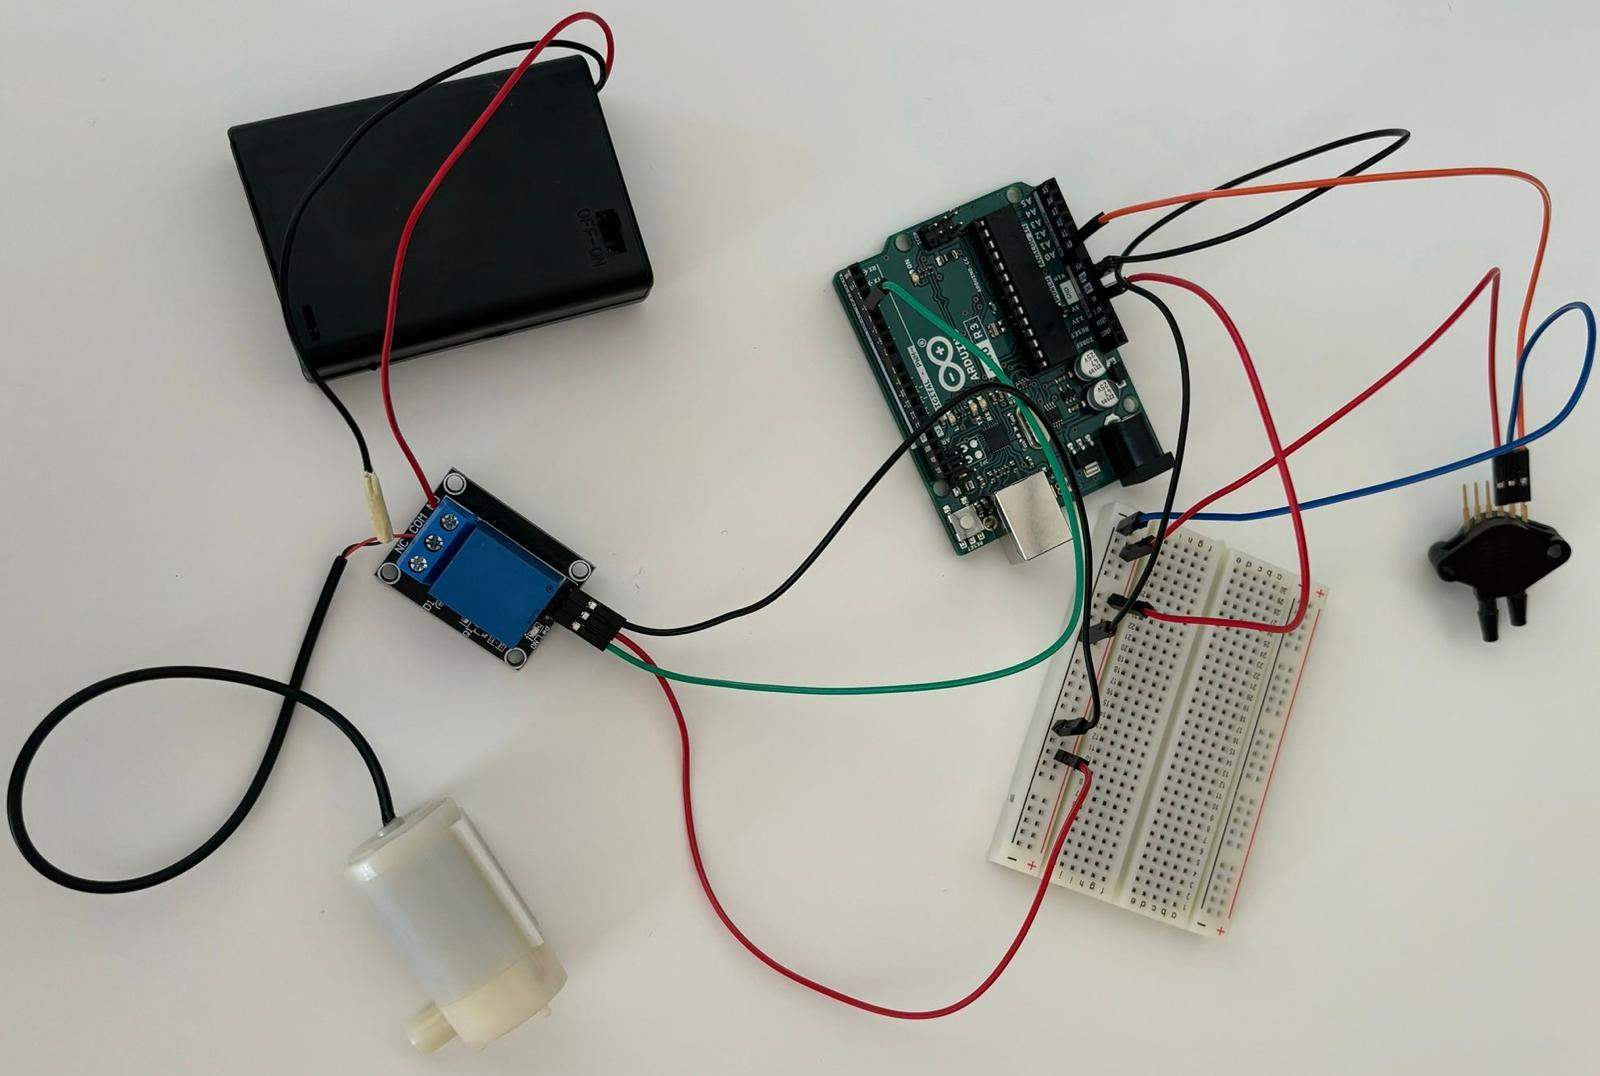
\includegraphics[width=0.9\textwidth]{img/circuitocompleto.jpg}
    \caption{Circuito electrónico. Imagen propia}
    \label{fig:circuito}
\end{figure}

El sensor se ha conectado de la siguiente manera. Su pinado consta de 6 pines, el pin 1 es el que presenta una muesca en la parte superior y va conectado a un pin analógico, A0 por ejemplo (cable azul). El pin 2 va conectado a GND (cable negro) y el pin 3 a 5V (cable rojo). Estas conexiones las podemos observar detalladamente en la Figura \ref{fig:conex_sens}.
\begin{figure}[h]
    \centering
    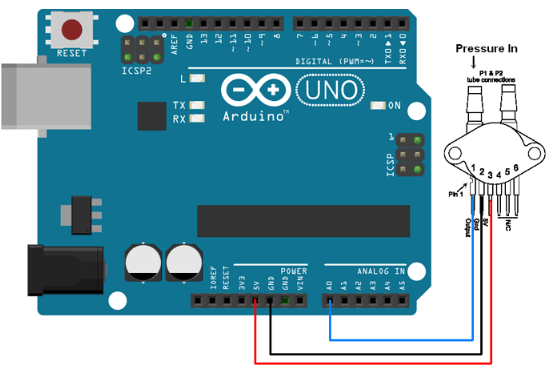
\includegraphics[width=0.9\textwidth]{img/conexion_sensr.PNG}
    \caption{Conexión sensor NPX MPX5010DP \cite{conexsen}}
    \label{fig:conex_sens}
\end{figure}

El relé, la mini bomba y la batería se han conectado entre ellas a la placa de Arduino. El relé es el encargado de hacer de interruptor, encendiendo y apagando la mini bomba, y la batería es necesaria para el suministro de corriente. El relé cuenta con tres pines y tres contactos. Los pines van conectados a la placa. El pin con el cable verde, va conectado a un pin digital, el del medio, cable rojo, a 5V y el siguiente, cable negro, a GND. Tanto la mini bomba como la batería cuentan con un cable rojo (+) y otro negro (-) cada una. El cable rojo de la mini bomba se introduce en el contacto común (C) del relé. Para ello es necesario utilizar un destornillador para aflojar un poco el tornillo y una vez introducido el cable lo apretamos para que se quede fijo y no se salga. Es importante que el cable que quede fuera del relé esté completamente aislado para que no ocurran cortocircuitos. El contacto común es el que se moverá abriendo o cerrando el circuito cuando se aplique corriente a la bobina y se genere el campo electromagnético, por eso el cable que debe ir ahí conectado es el del dispositivo que queremos controlar, en este caso, la mini bomba. El cable rojo de la batería irá al contacto normalmente abierto (NO) o al normalmente cerrado (NC), indistintamente. Por último se empalmarán los cables negros de la mini bomba y la batería, y quedarán juntos y correctacmente aislados. Para realizar el empalme sirve con quitar un poco del aislante que les recubre y entrelazar los filamentos entre ellos para que se produzca el contacto. En la Figura \ref{fig:conex_rele} podemos observar la conexión de estos tres componentes junto con la placa de Arduino.
\begin{figure}[h]
    \centering
    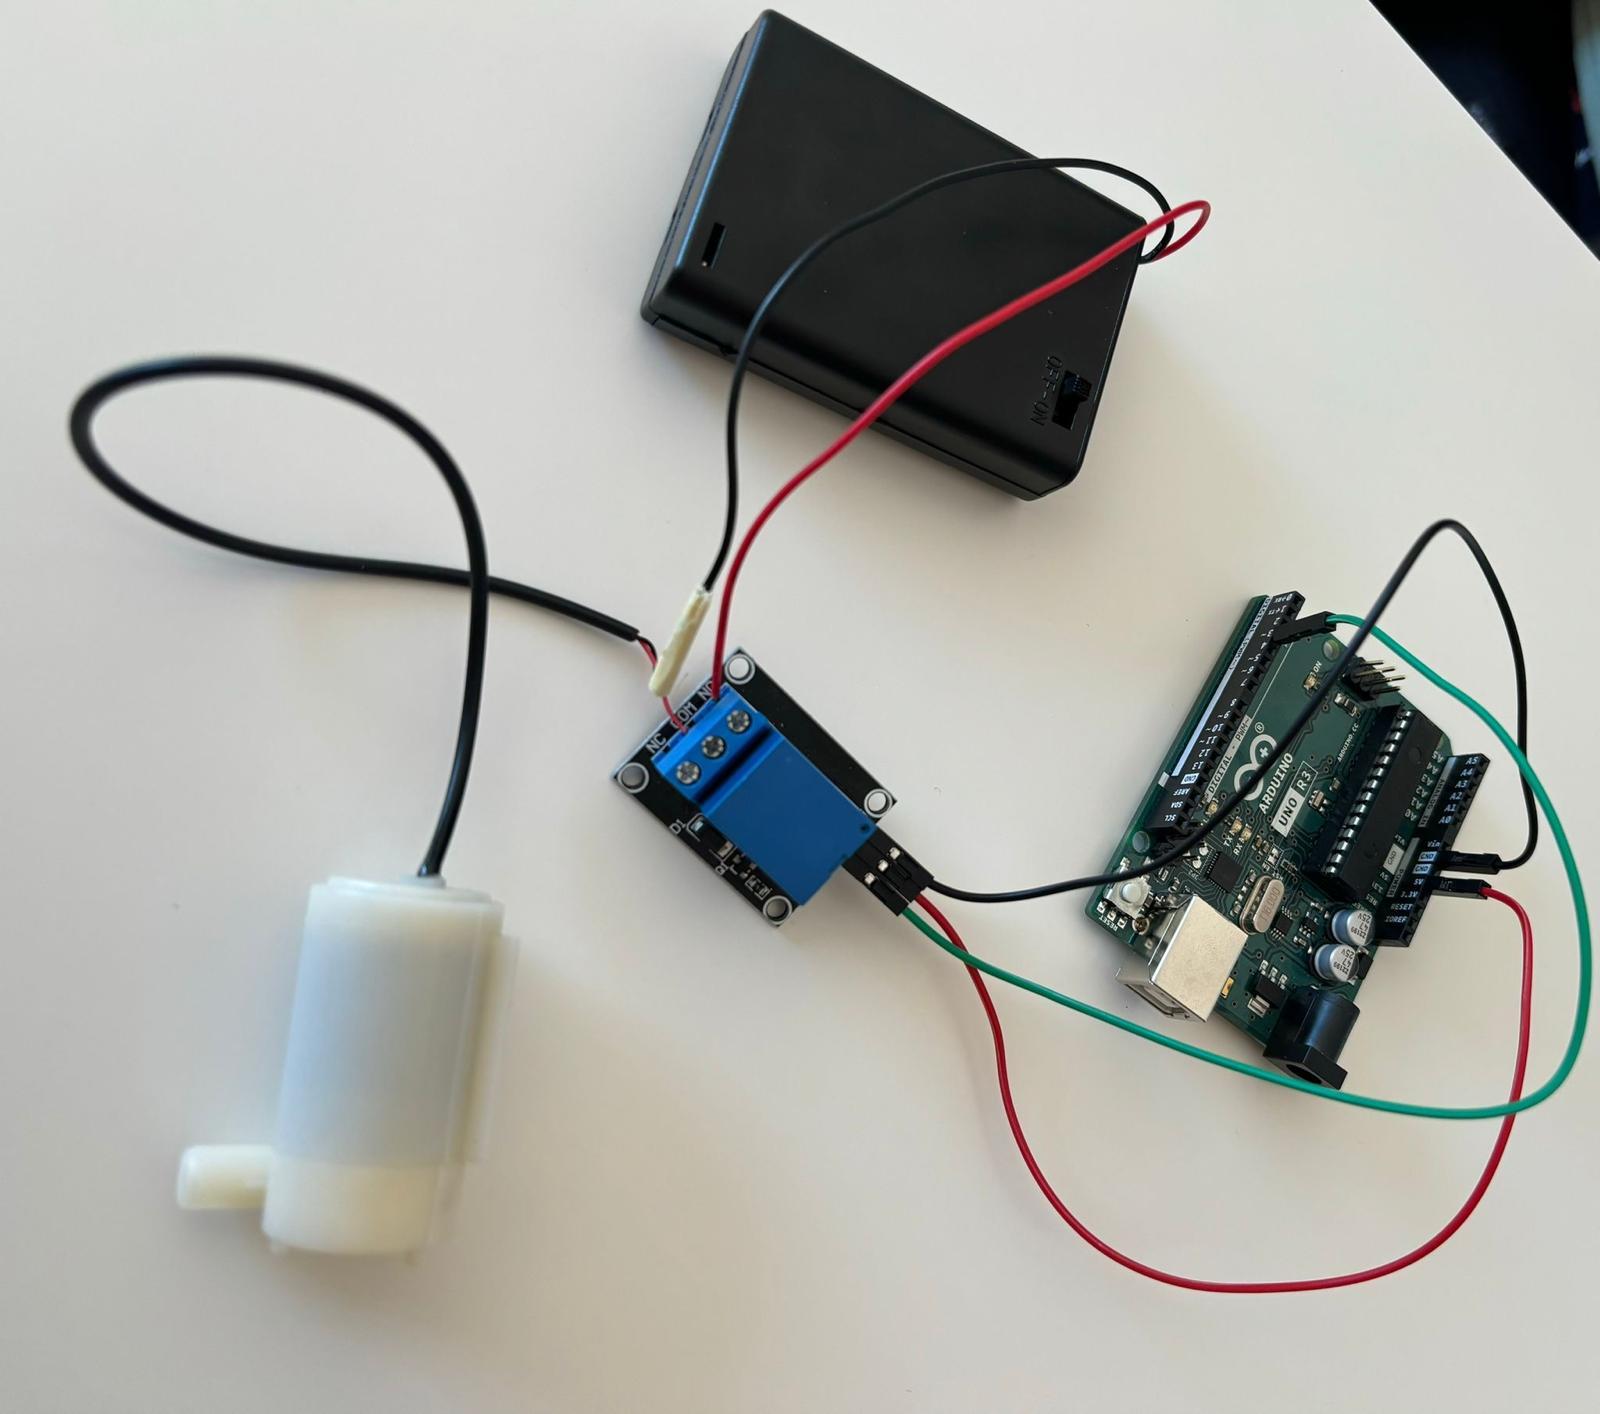
\includegraphics[width=0.9\textwidth]{img/rele-bomba.jpg}
    \caption{Conexión del relé, mini bomba y batería. Imagen propia}
    \label{fig:conex_rele}
\end{figure}

Con todo el circuito eléctrico montado, el último paso antes de conectarlo al ordenador, es colocar la manguera en la mini bomba y crear un colchón de aire al sensor (debido a que no se puede mojar) a través del empleo de otra manguera, tubo de plástico transparente, que irá introducido dentro del agua. El montaje del circuito completo lo podemos observar en la Figura \ref{fig:completo}.
\begin{figure}[H]
    \centering
    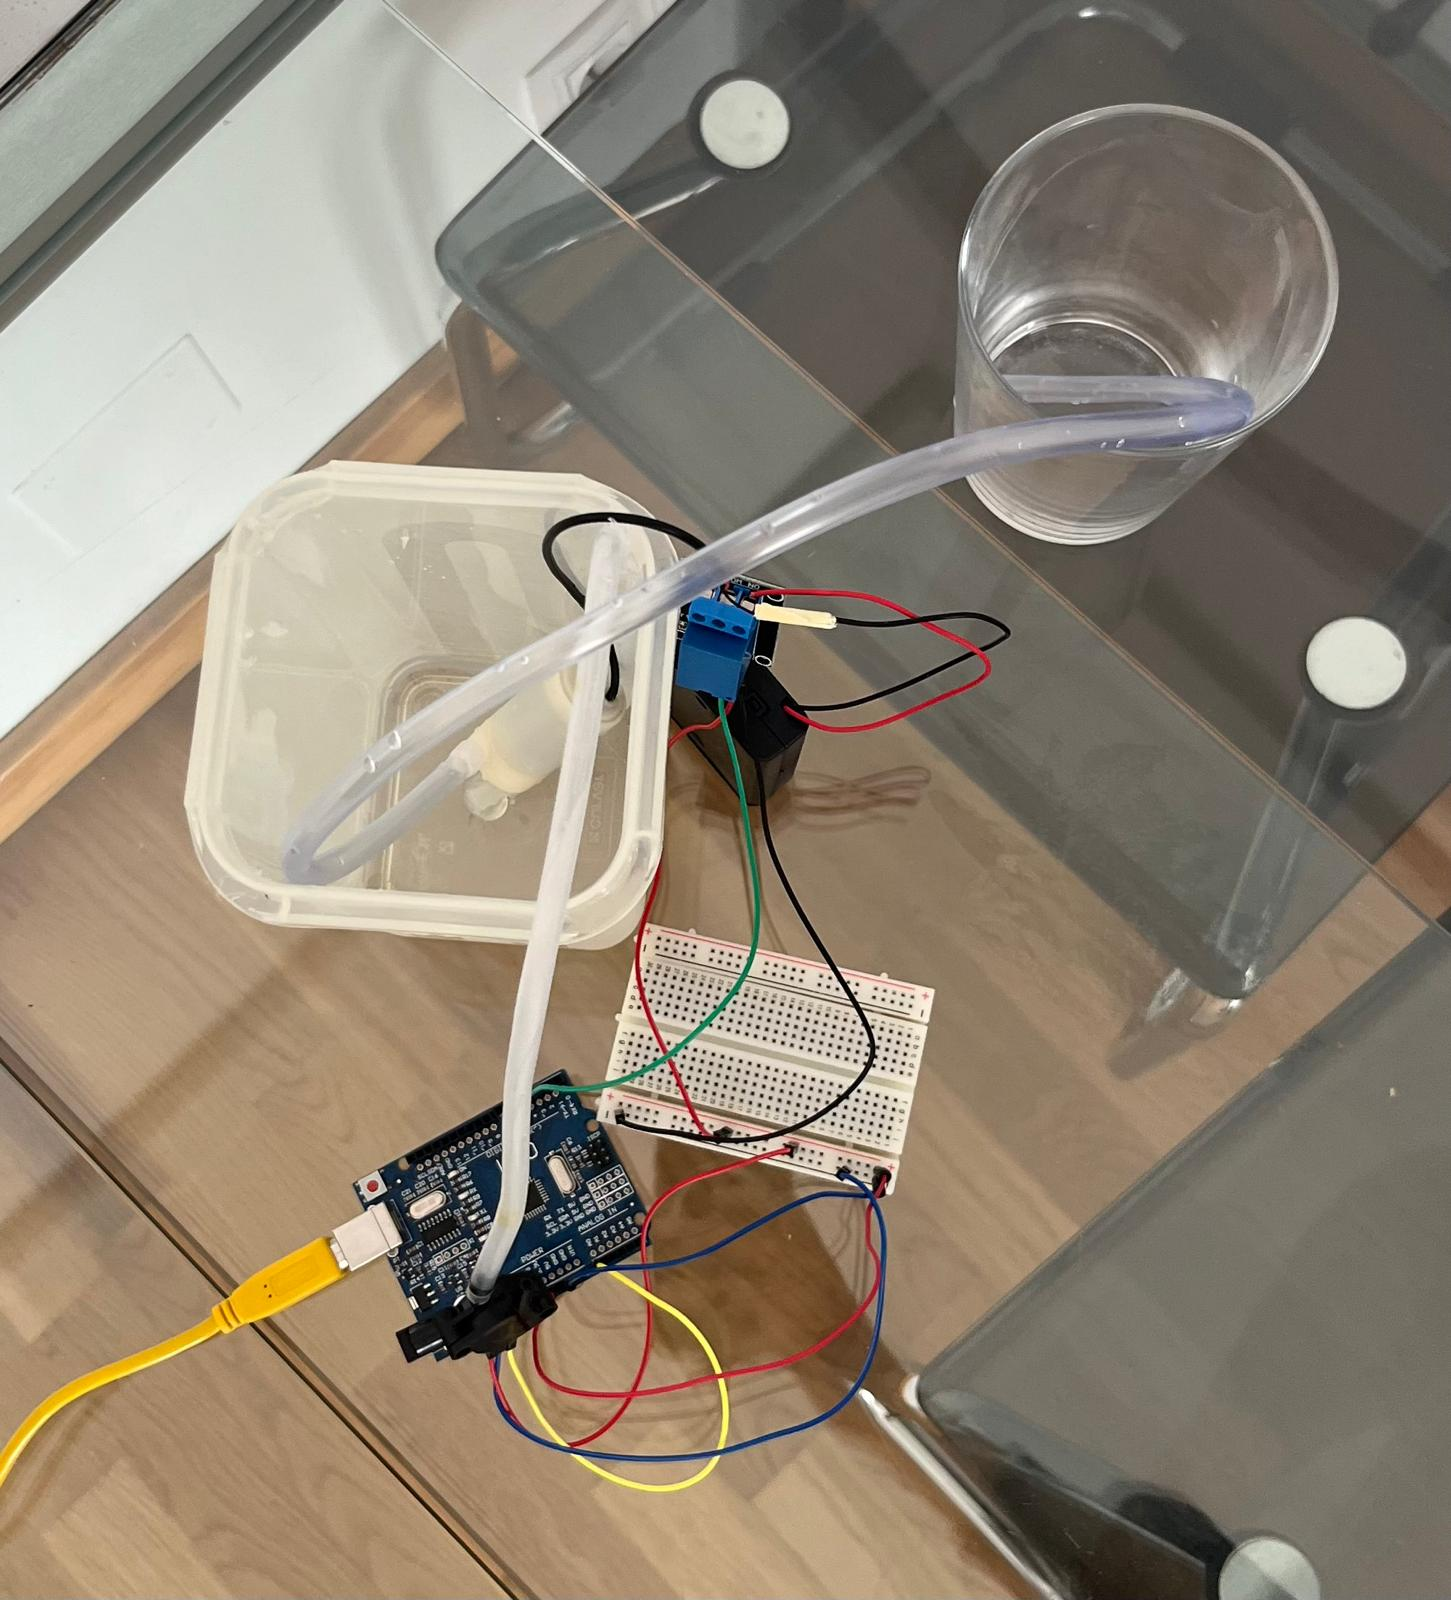
\includegraphics[width=0.8\textwidth]{img/conexioncontanques.jpg}
    \caption{Circuito completo con tanques. Imagen propia }
    \label{fig:completo}
\end{figure}


Una vez tengamos todo listo, haremos uso del cable USB para conectar la placa de Arduino al ordenador y ejecutar el programa. Podemos ver el código desarrollado en el Repositorio, en la carpeta Arduino encontraremos un archivo con el nombre  \textit{code-sensor.ino}, no obstante, se muestra a continuación:
\begin{lstlisting}
// Conexion de los pines del sensor y el rele
const int pinSensor = A0; // El sensor esta conectado al pin analogico A0
const int rele = 4; // El rele esta conectado al pin digital 4

// Variables para realizar las lecturas del sensor
double Vs = 5.0; // Voltaje de alimentacion del sensor --> 5V
double Vout; //Voltaje de salida
double P;
double P1;
double P2;
double Tol = 0.48; // Ajuste para calibrar la medida del sensor

// Datos solicitados
String nombreCompleto = "";
int anoNacimiento = 0;
String usuario = "";
String contrasena = "";
bool datosCompletos = false; //Variable booleana para controlar si los datos han sido completados y asi poder empezar a realizar las lecturas


bool bombaActivada = false; //Variable booleana para controlar si la minibomba se ha activado

void setup() {
  Serial.begin(9600);

  pinMode(rele, OUTPUT); //Configuracion del rele como salida
  digitalWrite(rele, LOW); //Inicialmente el rele esta apagado
  
  Serial.println("Por favor, introduce tu nombre completo:"); // Solicita los datos al usuario
}

void loop() {
  if (!datosCompletos) {
    //Entrada de datos por pantalla
    if (Serial.available() > 0) {
      if (nombreCompleto == "") {
        nombreCompleto= Serial.readStringUntil('\n');
        Serial.print("Nombre completo: ");
        Serial.println(nombreCompleto);
        Serial.println("Introduce tu ano de nacimiento:");
      } else if (anoNacimiento == 0) {
        anoNacimiento= Serial.readStringUntil('\n').toInt();
        if (anoNacimiento > 2006) {
          Serial.println("Error: Debe ser mayor de edad. Introduce nuevamente:");
          anoNacimiento=0; //Reinicio del ano para volver a introducirlo
        } else {
          Serial.print("Ano de nacimiento: ");
          Serial.println(anoNacimiento);
          Serial.println("Introduce tu usuario (DNI sin letras):");
        }
      } else if (usuario == "") {
        usuario = Serial.readStringUntil('\n');
        if (usuario.length() != 8) { //El DNI tiene 8 cifras
          Serial.println("Error: El usuario debe contener exactamente 8 caracteres. Introduce nuevamente:");
          usuario = ""; // Reinicia el usuario para volver a introducirlo
        } else {
          Serial.print("Usuario: ");
          Serial.println(usuario);
          Serial.println("Introduce tu contrasena (exactamente 8 caracteres):");
        }
      } else if (contrasena == "") {
        contrasena = Serial.readStringUntil('\n');
        if (contrasena.length() != 8) {
          Serial.println("Error: La contrasena debe tener 8 caracteres. Introduce nuevamente:");
          contrasena = ""; // Reinicia la contrasena para volver a introducirlo
        } else {
          Serial.print("Contrasena: ");
          for (int i = 0; i < contrasena.length(); i++) { //Bucle for para contar los caracteres introducimos y ponerlos con *
            Serial.print('*');
          }
          Serial.println();
          datosCompletos = true; //Variable booleana a true cuando los datos esten completos y correctos
          Serial.println("Datos completados. El sensor comenzara a realizar las lecturas.");
        }
      }
    }
  } else if (!bombaActivada) {
    Vout = float(analogRead(pinSensor)) * 5.0 / 1023.; // Lectura del voltaje con analogRead() --> Leemos lo que hay en el pin A0 (V)
    P = (Vout - 0.04 * Vs) / (0.09 * Vs); // Calculamos la presion (Figura 4 datasheet) kPa
    P1 = P * 7.50062; // P1 es la presion en mmHg 1kPa = 7.50062mmHg 
    P2= P1 + Tol; 

   
    Serial.print("\n\nVoltaje:");
    Serial.print(Vout);
    Serial.println(" V");
    Serial.print("Presion:");
    Serial.print(P2);
    Serial.println(" mmHg");

    if (P2 > 4.0 && !bombaActivada) { //Cuando se detecten valores superiores a 4 mmHg --> abrir mini bomba
      Serial.println("Se han detectado valores altos de presion, activando mini bomba...");
      digitalWrite(rele, HIGH); //Activa el rele para encender la minibomba
      delay(3000); 
      digitalWrite(rele, LOW); //Desactiva el rele para apagar la minibomba
      Serial.println("Mini bomba desactivada.");
      bombaActivada = true; 
      Serial.println("Prueba completada.");
    }

    delay(1000);
  }
}
\end{lstlisting}


El primer paso después de conectar la placa será compilar y subir el código. A continuación, acceder al monitor y comenzar a introducir los datos solicitados. En la Figura \ref{fig:verificar} tenemos el orden de verificación, subida y acceso al monitor respectivamente.
\begin{figure}[h]
    \centering
    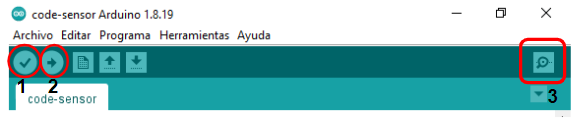
\includegraphics[width=1\textwidth]{img/compilar.PNG}
    \caption{(1) verificar, (2) subir y (3) monitor. Imagen propia }
    \label{fig:verificar}
\end{figure}


\section{Manuales y/o Demostraciones prácticas}
 Este apartado está dedicado a mostrar las demostraciones prácticas del proyecto. Una vez conectado el circuito y verificado y subido el código, procedemos a la apertura del monitor y comenzamos a completar los datos que se piden por pantalla. Primero el nombre completo (nombre y apellidos), después el año de nacimiento, usuario y por último la contraseña. En las Figuras \ref{fig:monitorINICIAL}, \ref{fig:monitorNOMBRE}, \ref{fig:monitorAÑO}, \ref{fig:monitorUSUARIO}, \ref{fig:monitorCONTRASEÑA} y \ref{fig:monitorCOMPLETO}  podemos observar este procedimiento.
 %MONITOR INICIAL
 \begin{figure}[H]
    \centering
    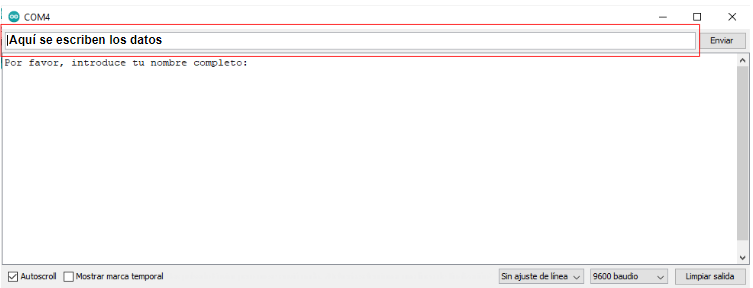
\includegraphics[width=1.3\textwidth]{img/monitorvacio.PNG}
    \caption{Estado inicial del monitor. Imagen propia }
    \label{fig:monitorINICIAL}
\end{figure}

%MONITOR NOMBRE
 \begin{figure}[H]
    \centering
    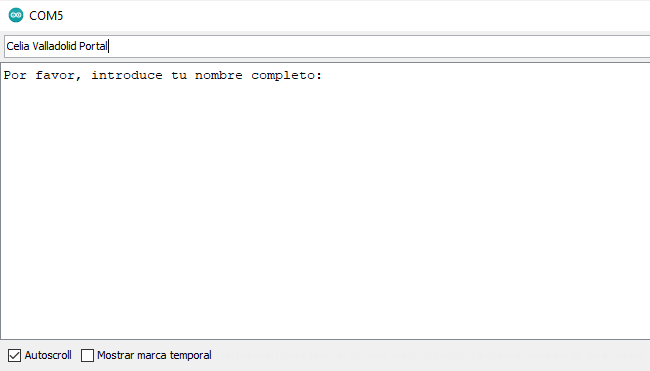
\includegraphics[width=1.1\textwidth]{img/monitornombre.PNG}
    \caption{Monitor: nombre completo. Imagen propia }
    \label{fig:monitorNOMBRE}
\end{figure}

%MONITOR AÑO
 \begin{figure}[H]
    \centering
    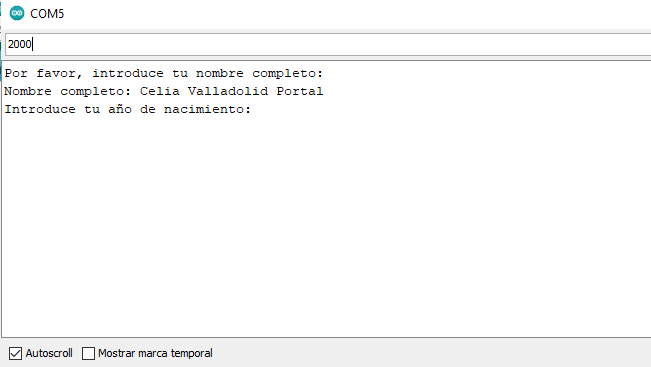
\includegraphics[width=1.1\textwidth]{img/monitoraño.PNG}
    \caption{Monitor: año de nacimiento. Imagen propia }
    \label{fig:monitorAÑO}
\end{figure}

%MONITOR USUARIO
 \begin{figure}[H]
    \centering
    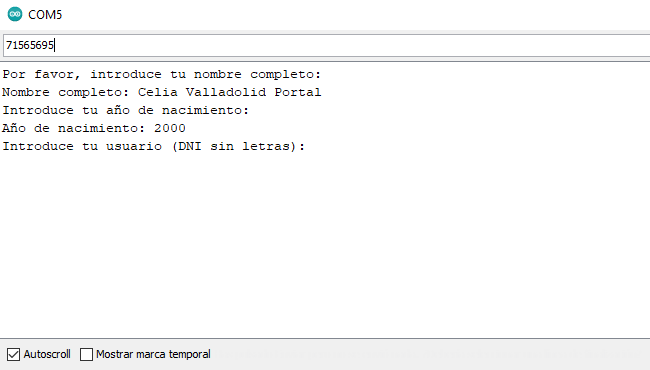
\includegraphics[width=1.1\textwidth]{img/monitorusuario.PNG}
    \caption{Monitor: usuario. Imagen propia }
    \label{fig:monitorUSUARIO}
\end{figure}

%MONITOR CONTRASEÑA
 \begin{figure}[H]
    \centering
    \includegraphics[width=1.1\textwidth]{img/monitorcontraseña.PNG}
    \caption{Monitor: contraseña. Imagen propia }
    \label{fig:monitorCONTRASEÑA}
\end{figure}

%MONITOR CON DATOS COMPLETOS
 \begin{figure}[H]
    \centering
    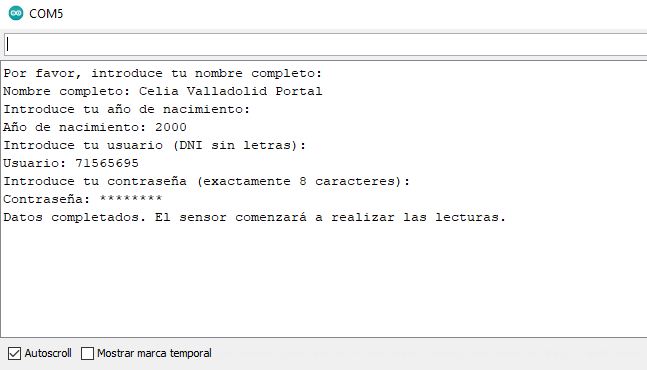
\includegraphics[width=1.1\textwidth]{img/monitorcompleto.PNG}
    \caption{Monitor con datos completos. Imagen propia }
    \label{fig:monitorCOMPLETO}
\end{figure}

Algunos campos como el año de nacimiento, el usuario y la contraseña, presentan alguna condición. Respecto al año de nacimiento, actualmente no puede ser superior a 2006, es decir, el usuario deberá de ser mayor de edad. La longitud tanto del usuario como de la contraseña será de 8 caracteres. En el caso del usuario es debido a que se corresponde con el DNI sin letra, sumando un total de 8 cifras y en el caso de la contraseña es simplemente por fijar una determinada longitud. Si alguna de estas condiciones no se cumpliera a la hora de ingresar los datos, el sistema se lo hará saber al usuario a través de un mensaje de error, ofreciéndole la oportunidad de introducir de nuevo el dato por si anteriormente hubo una confusión. Lo podemos observar en las Figuras \ref{fig:monitorAÑOMAL}, \ref{fig:monitorERRORAÑO}, \ref{fig:monitorUSUARIOMAL}, \ref{fig:monitorERRORUSUARIO}, \ref{fig:monitorCONTRASEÑAMAL}, \ref{fig:monitorERRORCONTRASEÑA} y \ref{fig:monitorFINAL} .

%MONITOR CON AÑO MAL
 \begin{figure}[h]
    \centering
    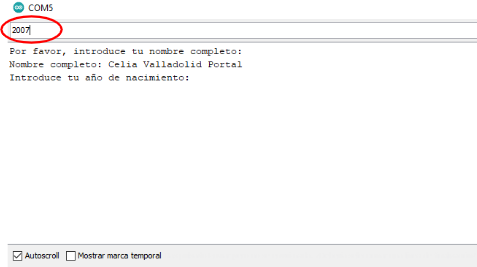
\includegraphics[width=1.1\textwidth]{img/monitorañomal.PNG}
    \caption{Monitor: introducción incorrecta del año, superior a 2006. Imagen propia }
    \label{fig:monitorAÑOMAL}
\end{figure}

%MONITOR ERROR AÑO
 \begin{figure}[h]
    \centering
    \includegraphics[width=1.1\textwidth]{img/monitorerroraño.PNG}
    \caption{Monitor: mensaje de error e introducción válida del año. Imagen propia }
    \label{fig:monitorERRORAÑO}
\end{figure}

%MONITOR CON USUARIO MAL
 \begin{figure}[h]
    \centering
    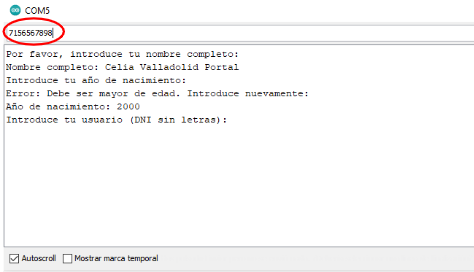
\includegraphics[width=1.1\textwidth]{img/monitorusuariomal.PNG}
    \caption{Monitor: introducción incorrecta de usuario, longitud distinta de 8. Imagen propia }
    \label{fig:monitorUSUARIOMAL}
\end{figure}

%MONITOR ERROR USUARIO
 \begin{figure}[h]
    \centering
    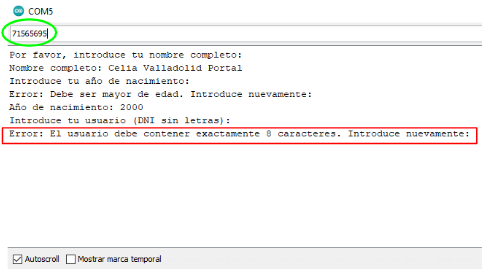
\includegraphics[width=1.1\textwidth]{img/monitorerrorusuario.PNG}
    \caption{Monitor: mensaje de error e introducción válida del usuario. Imagen propia }
    \label{fig:monitorERRORUSUARIO}
\end{figure}

%MONITOR CON CONTRASEÑA MAL
 \begin{figure}[h]
    \centering
    \includegraphics[width=1.1\textwidth]{img/monitorcontraseñamal.PNG}
    \caption{Monitor: introducción incorrecta de contraseña, longitud distinta de 8. Imagen propia }
    \label{fig:monitorCONTRASEÑAMAL}
\end{figure}

%MONITOR ERROR CONTRASEÑA
 \begin{figure}[h]
    \centering
    \includegraphics[width=1.1\textwidth]{img/monitorerrorcontraseña.PNG}
    \caption{Monitor: mensaje de error e introducción válida de contraseña. Imagen propia }
    \label{fig:monitorERRORCONTRASEÑA}
\end{figure}

%MONITOR FINAL
 \begin{figure}[h]
    \centering
    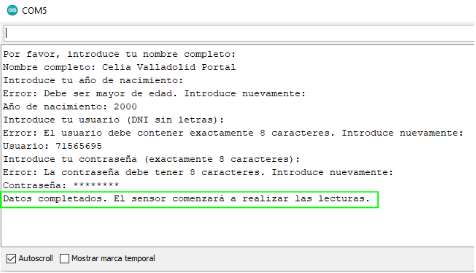
\includegraphics[width=1.1\textwidth]{img/monitorfinalbien.PNG}
    \caption{Monitor con datos completos. Imagen propia }
    \label{fig:monitorFINAL}
\end{figure}
\clearpage
Con los datos completos, el sensor comenzará a realizar lecturas de presión, detectando cambios y determinando cuando debe de activar la mini bomba para derivar el fluido de un tanque a otro.

Todas las demostraciones están contenidas en la carpeta demostraciones del Repositorio.
